%BEGIN COPYPASTE EL INFORME DEL INFO
\documentclass[10pt, a4paper,english,spanish]{article}
\usepackage{subfig}

\parindent=20pt
\parskip=8pt
\usepackage[width=15.5cm, left=3cm, top=2.5cm, height= 24.5cm]{geometry}

\usepackage{ccfonts,eulervm} 
\usepackage[T1]{fontenc}
\usepackage{epigraph}
\usepackage{amsmath}
\usepackage{amsfonts}
\usepackage{amssymb}
\usepackage{fancyhdr}
\usepackage[activeacute, spanish]{babel}
\usepackage{cancel}
\usepackage[utf8]{inputenc}
\usepackage{algorithm}
\usepackage{algpseudocode}
\usepackage{afterpage}
\usepackage{caratula}
\usepackage{url}
\usepackage{fancyhdr}
\usepackage{listings}
\usepackage{ulem}
\usepackage{dashrule}
\usepackage{fancyvrb}
\usepackage{pdflscape}

\floatname{algorithm}{Algoritmo}

\newtheorem{theorem}{Teorema}[section]
\newtheorem{lemma}[theorem]{Lema}
\newtheorem{proposition}[theorem]{Proposici\'on}
\newtheorem{corollary}[theorem]{Corolario}

\newcommand{\Var}{\textbf{var }}
\newcommand{\True}{\textbf{true }}
\newcommand{\False}{\textbf{false }}
\newcommand{\Break}{\textbf{break }}
\newcommand{\Continue}{\textbf{continue }}
\newcommand{\Param}{\textbf{param }}

\newenvironment{proof}[1][Demostraci\'on]{\begin{trivlist}
\item[\hskip \labelsep {\bfseries #1}]}{\end{trivlist}}
\newenvironment{definition}[1][Definici\'on]{\begin{trivlist}
\item[\hskip \labelsep {\bfseries #1}]}{\end{trivlist}}
\newenvironment{example}[1][Ejemplo]{\begin{trivlist}
\item[\hskip \labelsep {\bfseries #1}]}{\end{trivlist}}
\newenvironment{remark}[1][Observaci\'on]{\begin{trivlist}
\item[\hskip \labelsep {\bfseries #1}]}{\end{trivlist}}

\newcommand{\qed}{\nobreak \ifvmode \relax \else
      \ifdim\lastskip<1.5em \hskip-\lastskip
      \hskip1.5em plus0em minus0.5em \fi \nobreak
      \vrule height0.75em width0.5em depth0.25em\fi}

\algrenewcommand{\algorithmiccomment}[1]{//\textit{#1} }

\lstset{language=sql,numbers=left,tabsize=2,
	morekeywords={BEGIN,DECLARE,FOR,CREATE,PROCEDURE,RAISEERROR,EACH,ROW,BEFORE,AFTER,MINUS,IF},
	breaklines=true,breakatwhitespace=true}

\pagestyle{fancy}
\thispagestyle{fancy}
\addtolength{\headheight}{1pt}
\lhead{BD - TP2}
\rhead{Grupo 1}
\cfoot{\thepage}
\renewcommand{\footrulewidth}{0.4pt}
\newcommand{\hblacksquare}{\hfill \blacksquare}
%FIN COPYPASTE EL INFORME DEL INFO
\begin{document}

\materia{Bases de datos}
\submateria{Primer Cuatrim\'estre de 2013}
\titulo{Trabajo Pr\'actico 2}
\subtitulo{Informe}
\grupo{Grupo 1}
\integrante{Pablo Gauna}{334/09}{gaunapablo@gmail.com}
\integrante{Julián Sackmann}{540/09}{jsackmann@gmail.com}
\integrante{Manuel Ferreria}{199/10}{m.ferreria@gmail.com}
\integrante{Juan Pablo Darago}{272/10}{jpdarago@gmail.com}

\maketitle
\pagebreak

\tableofcontents
\pagebreak

\section{Investigación sobre Oracle}

Desde su versión 8i, el motor de base de datos \texttt{Oracle} utiliza tres buffer pools para tener bloques de datos. Un resumen sucinto de la arquitectura de buffers en \texttt{Oracle} puede verse en la figura \ref{fotito}.

\begin{figure}[H]\centering
	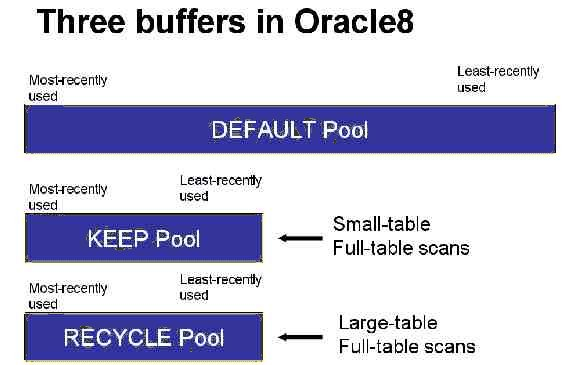
\includegraphics[scale=0.5]{keepRecycle.jpg}
	\caption{Los tres buffers de \texttt{Oracle 8i}}
	\label{fotito}
\end{figure}
\subsection{Uso}
Para utilizar los distintos buffer pools, se marcan objetos de la base de datos de tal forma que quedan asociados a un pool particular. Luego de esto, todos los bloques asociados a ese objeto (un bloque no puede tener elementos de distintos objetos) irá siempre a ese buffer\footnote{http://docs.oracle.com/cd/B10500\_01/server.920/a96533/memory.htm}. 

Es digno observar que estos buffers no tienen un comportamiento automático. Es el usuario quien debe encargarse de marcar qué páginas irán a qué buffer para que los buffers acá definidos sean utilizados. 

\subsubsection{Ejemplo}
\begin{Verbatim}[xleftmargin=-3em]
	CREATE TABLE t1 (
		my_date   DATE NOT NULL,
		my_number NUMBER(12,10) NOT NULL,
		my_row    NUMBER(12) NOT NULL)
	STORAGE (BUFFER_POOL KEEP);	
\end{Verbatim}

\subsection{Default pool}
Es el espacio de memoria que se utiliza por defecto para los bloques que pertenecen a objetos que no fueron marcados específicamente para ser usados con otras tablas.

\newpage

\subsection{Keep pool}
El buffer \texttt{keep} se usa para almacenar bloques pertenecientes a tablas e índices que son utilizados muy frecuentemente. 

Este buffer pool es particularmente eficiente a la hora de ``proteger'' a los bloques de memoria más frecuentemente utilizados de los nocivos efectos de desalojo masivo que tienen las implementaciones más triviales de \textit{full table scan}. Generalmente, al realizar una de estas consultas se requiere mucha memoria, lo que termina forzando que un gran número de bloques de tablas frecuentemente utilizadas sean descartadas y sea necesario volver a traerlos de disco si se quieren volver a utilizar. Es por esto que \texttt{Oracle} permite marcar tablas para que estas vayan al buffer \texttt{keep}. De esta forma se intenta evitar su pérdida cuando deben ser desalojados por alguna query.

Notar que este método no es 100\% efectivo, dado que muy probablemente la suma de los bloques de todas las tablas marcadas como \texttt{keep} (así sea una sola) supere el tamaño del buffer. Con lo cual en algún momento es posible que sea necesario guardar un bloque en el buffer \texttt{keep} cuando este esté lleno, con lo que va a tener que descartarse algún bloque mediante alguna política de reemplazo (en \texttt{Oracle}, generalmente \textit{LRU}). 

En general se recomienda que el buffer \texttt{keep} sea utilizado para objetos pequeños\footnote{http://www.exploreoracle.com/2009/04/02/keep-buffer-pool-and-recycle-buffer-pool/}.

\subsection{Recycle pool}
A diferencia del \texttt{keep} buffer, el \texttt{recycle} buffer debe ser utilizado con bloques pertenecientes a tablas que son raramente accedidos. Los bloques que están en este pool son descartados rápidamente una vez que dejan de ser utilizados\footnotemark[\value{footnote}]. Esto es porque en Oracle existe una opción \textit{ASM} que, usada en este caso, permite realocar la memoria del \texttt{recycle} a otro componente del SGA (\textit{System Global Area}, un componente que forma parte del sistema de administración de memoria del DBMS).

Por recomendación de \texttt{Oracle}\footnote{http://docs.oracle.com/cd/B28359\_01/server.111/b28274/memory.htm\#autoId29}, el tamaño del \texttt{recycle} pool debe ser lo suficientemente chico como para no ocupar RAM que podría ser mejor destinada a otro pool (como lo bloques se desalojan relativamente rápido, es mucho mejor usado el espacio en el default o \texttt{keep} pool), pero lo suficientemente grande como para que un bloque no sea desalojado en medio de una transacción (supongamos una transacción que levanta un bloque de un objeto marcado de \texttt{recycle}, luego lo procesa junto con otros y luego lo escribe. Si el \texttt{recycle} buffer es demasiado pequeño y fue necesario desalojar el bloque durante el procesado, a la hora de grabarlo va a ser necesario volver a levantarlo, lo que es mucho más ineficiente).

Históricamente (en \texttt{Oracle 8}), el \texttt{recycle} pool comenzó como un buffer donde alojar bloques \textit{transitorios}\footnote{http://www.praetoriate.com/t\_\%20tuning\_recycle\_pool.htm}. Un bloque \textit{transitorio} es aquel que se lee como parte de un \textit{full table scan} y es poco probable que vuelva a ser utilizado en el futuro cercano. Este concepto luego fue extendido de bloques transitorios a cualquier bloque perteneciente a objetos particulares que el dba sepa que serán utilizados muy esparsamente.

\newpage

\section{Implementaci\'on}

\subsection{Catalog Manager}

En primer lugar realizamos la implementaci\'on del manejador de c\'atalogo (\textit{Catalog Manager}). El propósito de este módulo es proveer datos para el resto de los módulos sobre las tablas de la base de datos. En particular se mantienen los siguientes datos sobre las tablas:

\begin{itemize}
	\item Identificador de tabla (que corresponde a un nombre de uso interno).
	\item Nombre de la tabla.
	\item El nombre de archivo que contendría los datos binarios de la tabla.
	\item El buffer al cual se deben asignar los datos de la tabla (valor opcional, se asigna un valor
	por \texttt{default} seg\'un la sem\'antica de buffers). 
\end{itemize}

La implementaci\'on del \textit{Catalog Manager} sigue la interfaz dada por la c\'atedra en \texttt{CatalogManager}. \texttt{CatalogManagerImpl} mantiene los cat\'alogos mediante el uso de archivos XML. A continuaci\'on presentamos un ejemplo de archivo:

\begin{Verbatim}[xleftmargin=-3em]
	<catalog>
		<table>
			<tableId>test.table</tableId>
			<tableName>A Test Table</tableName>
			<tablePath>testTable.table</tablePath>
			<tablePool>RECYCLE</tablePool>
		</table>
		<table>
			<tableId>test2.table</tableId>
			<tableName>Another Test Table</tableName>
			<tablePath>testTable2.table</tablePath>
		</table>
	</catalog>
\end{Verbatim}

Como se puede ver el formato es autoexplicativo: Se mantiene una secci\'on \textit{table} por cada tabla dentro de la cual se incluyen los datos pertinentes a esa tabla. Para facilitar el parseo todas las entradas para la informaci\'on de tablas se mantienen \textit{wrappeadas} en una secci\'on \texttt{catalog}.

El único rol de la clase \texttt{CatalogManagerImpl} es levantar el archivo XML indicado y parsear sus datos. Para ello decidimos utilizar la librer\'ia \texttt{JDOM 1.1}. Esta librer\'ia, si bien es de m\'as bajo nivel que \texttt{XStream}, su uso implica que no tenemos \textit{coupling} de nombres entre el formato del XML y los nombres de las propiedades de los descriptores de tabla (lo cual es requerido por la librer\'ia \texttt{XStream} antes mencionada por el uso de  \textit{reflection}). Utilizando esta librer\'ia de bajo nivel mantenemos separadas la representaci\'on en XML y la representaci\'on de los descriptores de tabla en c\'odigo en Java (porque para setearlos usamos sus \textit{accessor methods}).

Una vez levantado el cat\'alogo desde un archivo XML, la interfaz que provee permite, dada una tabla, obtener el descriptor de tabla. Esto lo hace instanciando un objeto de clase \texttt{Catalog}, que contiene una lista de \texttt{TableDescriptors}, la representaci\'on de descriptores de tabla. Este contiene todos los datos mencionados anteriormente. En caso de no existir un descriptor correspondiente a la tabla, se devuelve un valor nulo (\texttt{null} en Java).

Junto a la implementaci\'on se incluyen test de unidad de este m\'odulo. Los mismos est\'an realizados mediante el framework JUnit. Consisten en levantar el cat\'alogo de un archivo XML creado para el test y realizar luego una serie de verificaciones sobre los descriptores de tabla presentes, incluyendo casos borde como por ejemplo, un descriptor de tabla que no tiene especificado en el XML a que pool debe ir (el comportamiento para este caso es enviarla al buffer \texttt{DEFAULT}) y que el valor correspondiente a un descriptor de tabla que no existe es nulo.

\subsection{Multiple Buffer Manager}

Siguiendo la l\'inea de la investigaci\'on realizada anteriormente, implementamos el manejo de buffers usado por el motor \texttt{Oracle 11g} (aunque nos basamos principalmente en el sistema que viene implementado desde la versi\'on 8g).

Para lograr m\'as generalidad, decidimos implementar buffer pools multiples tal que puedan configurarse pools de nombres arbitrarios. Para ello, le permitimos al motor inicializar pools a partir de un diccionario \texttt{Map<String,Integer>} que nos permita obtener los nombres y tama\~nos correspondientes para cada buffer deseado.

La configuraci\'on del buffer usado como default decidimos tambi\'en dejarla al instanciador permitiendo pasarla como par\'ametro (a pesar de que se podr\'ia utilizar un nombre como DEFAULT, lo cual corresponde a la implementaci\'on de Oracle). Tambi\'en permitimos definir la estrategia de reemplazo de p\'aginas para usar en los buffers. Por simplicidad se decidi\'o que todos los buffers utilicen esta estrategia pasada como par\'ametro.

La implementaci\'on es sencilla, puesto que se pudo reutilizar mucho c\'odigo ya provisto: cada buffer pool se modela mediante un \texttt{SingleBufferPool}. Se mantiene un \texttt{Map<String,BufferPool>} que mapea $\text{nombre de pool} \rightarrow \text{instancia de pool}$. Estos mapeos se obtienen del cat\'alogo (que recibe el MultipleBufferPool de par\'ametro). La \'unica tarea del \texttt{MultipleBufferPool} por lo tanto es, dada una operaci\'on para una p\'agina, obtener el buffer correspondiente (que podría ser el DEFAULT si esta tabla no tiene asignado ningun pool) y realizar esa operaci\'on mediante la interfaz de \texttt{BufferPool} que posee \texttt{SingleBufferPool}.

Como se realizó anteriormente, se incluyen test de unidad para este m\'odulo realizados en JUnit. Para realizar los mismos se provee un \textit{mock} de la implementaci\'on de un cat\'alogo, que carga una lista est\'atica de descriptores.


\newpage

\section{Tests y Gráficos}
Para correr los tests y generar los gráficos se utilizó la función \textit{traceGenerator} provista en el motor para generar trazas válidas que utilizamos como inputs. 

Una vez generadas estas trazas corrimos el evaluador (también incluido en el código) y observamos el desempeño de nuestras implementaciones de single y múltiple buffer pools. Para realizar mediciones más precisas, comparamos los hit rates de acceso a disco considerando distintos accesos tales como BNLJ, INLJ, etc. Con esta información de los hit-rates generamos tablas con sus correspondientes los gráficos que se pueden ver en la sección \ref{secTablasYGraficos}.


\subsection{Tablas y Gráficos}\label{secTablasYGraficos}
\newpage

\section{Conclusiones}

En este trabajo pr\'actico se investig\'o el manejo de buffers como m\'odulo de un \textit{DBMS}, usando \texttt{UBADB} como plataforma de estudio. 

Se implement\'o la pol\'itica de \textit{Multiple Buffer Pools} bas\'andonos en la informaci\'on conocida del motor de bases de datos de \texttt{Oracle}, incluyendo adem\'as la implementaci\'on de un manejador b\'asico de cat\'alogo. 

Posteriormente a implementar y verificar la correctitud de estos m\'odulos (mediante tests de unidad) se procedi\'o a investigar y comparar esta estrategia de buffers contra la estrategia (ya implementada) de \textit{Single Buffer Pool} en una serie de casos de inter\'es. 

Se obtuvo que la performance del \textit{Multiple Buffer Pool} es similar o mejor a la del \textit{Single Buffer Pool} con una cantidad comparativa o incluso significativamente menor de recursos (en particular, se considero a este recurso como la cantidad de memoria principal necesaria). Concluimos entonces que la estrategia de \textit{Multiple Buffer Pools} es \'util para diversas situaciones, evitando con un gasto razonable de recursos la disminuci\'on de la \textit{performance} (en t\'erminos de accesos a disco por sobre accesos a memoria, que dada su diferencia de tiempo de acceso consideramos el \textit{hitrate} como una buena medici\'on de \textit{performance}).

\newpage

\section{Referencias}
\begin{itemize}
	\item http://www.dba-oracle.com/phys\_52.htm
	\item http://docs.oracle.com/cd/B10500\_01/server.920/a96533/memory.htm
	\item http://www.exploreoracle.com/2009/04/02/keep-buffer-pool-and-recycle-buffer-pool/
	\item http://docs.oracle.com/cd/B28359\_01/server.111/b28274/memory.htm\#autoId29
	\item http://www.praetoriate.com/t\_\ tuning\_recycle\_pool.htm
\end{itemize}

\end{document}
